\documentclass[11pt]{article}
\usepackage[margin=.5in]{geometry}
\usepackage[utf8]{inputenc}
\usepackage[T1]{fontenc}
\usepackage[french]{babel}
\usepackage{graphicx}
\usepackage[colorlinks]{hyperref}
\title{Révision intra\thanks{Ross : page du manuel en français -- Davignon : \href{https://dms.umontreal.ca/~davignon/MAT1720/notes_de_cours.pdf}{pdf}}}
\date{}
\setlength\parindent{0pt}

\begin{document}
	\maketitle
	\tableofcontents
	\newpage
	
	\section{Chapitre 5 : Variables aléatoires continues}
	\subsection{Ross auto-évaluation 5.6 p. 281}
	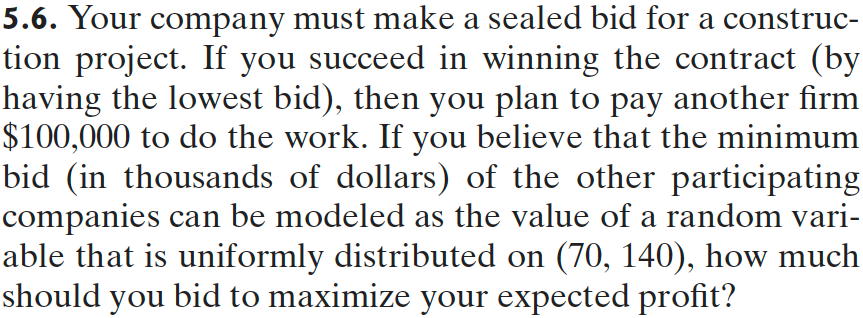
\includegraphics[width=.7\linewidth]{a5_6_p281}
	\newpage
	
	\subsection{Ross problème 5.22 p. 273}
	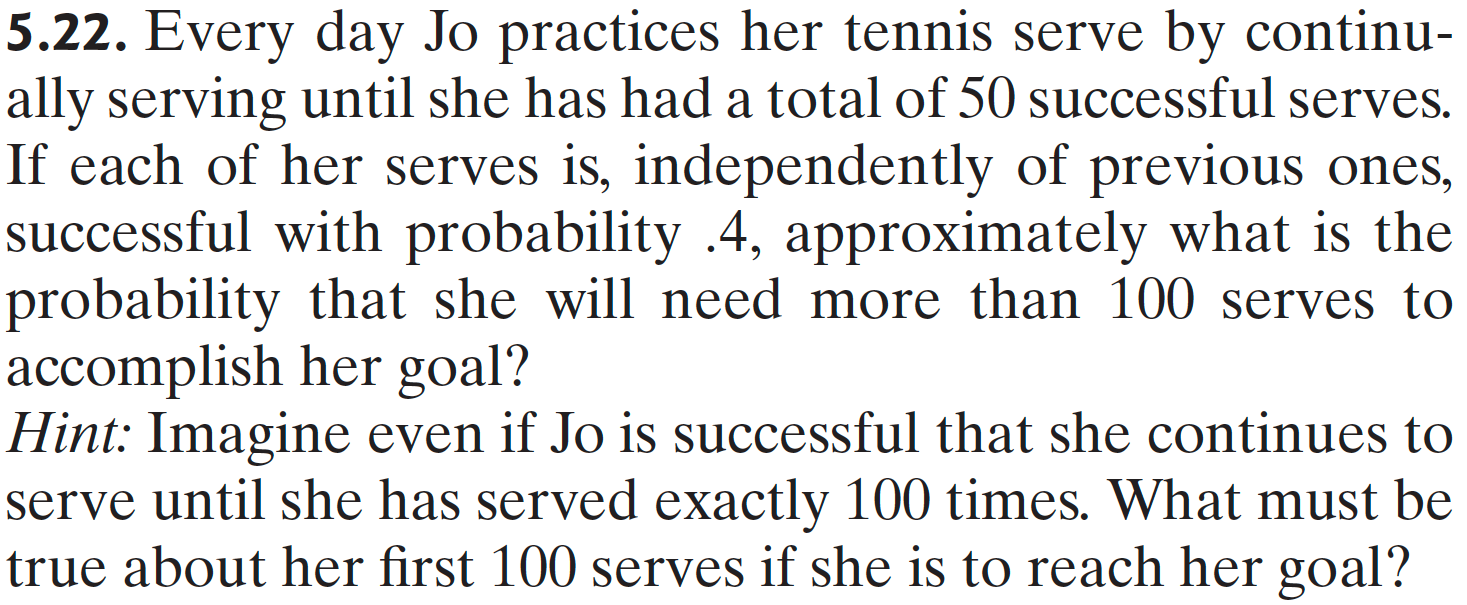
\includegraphics[width=.7\linewidth]{p5_22_p273}
	\newpage
	
	\subsection{Davignon exercice 5.7 p. 124}
	
\includegraphics[width=\linewidth]{dvg_5_7_p124}
	\newpage
	
	\subsection{Davignon exercice 5.4 p. 123}
	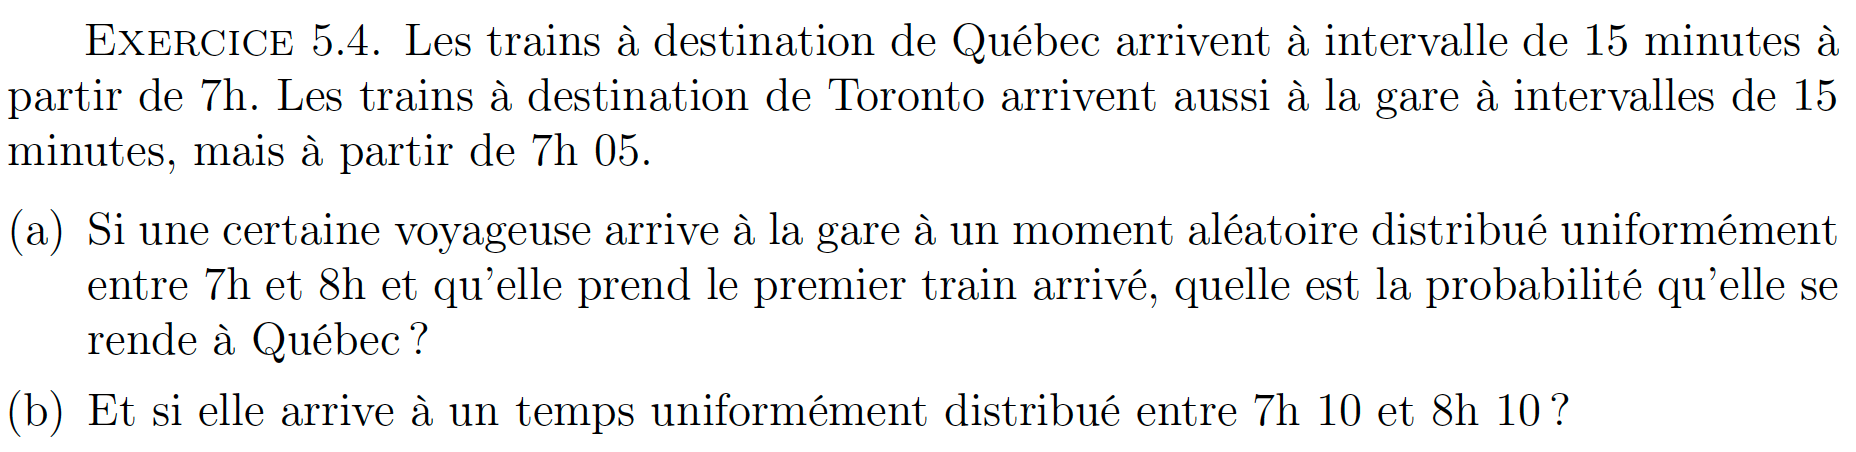
\includegraphics[width=\linewidth]{dvg_5_4_p123}
	\newpage
	
	\section{Chapitre 4 : Variables aléatoires}
	\subsection{Ross problème 4.29 p. 212}
	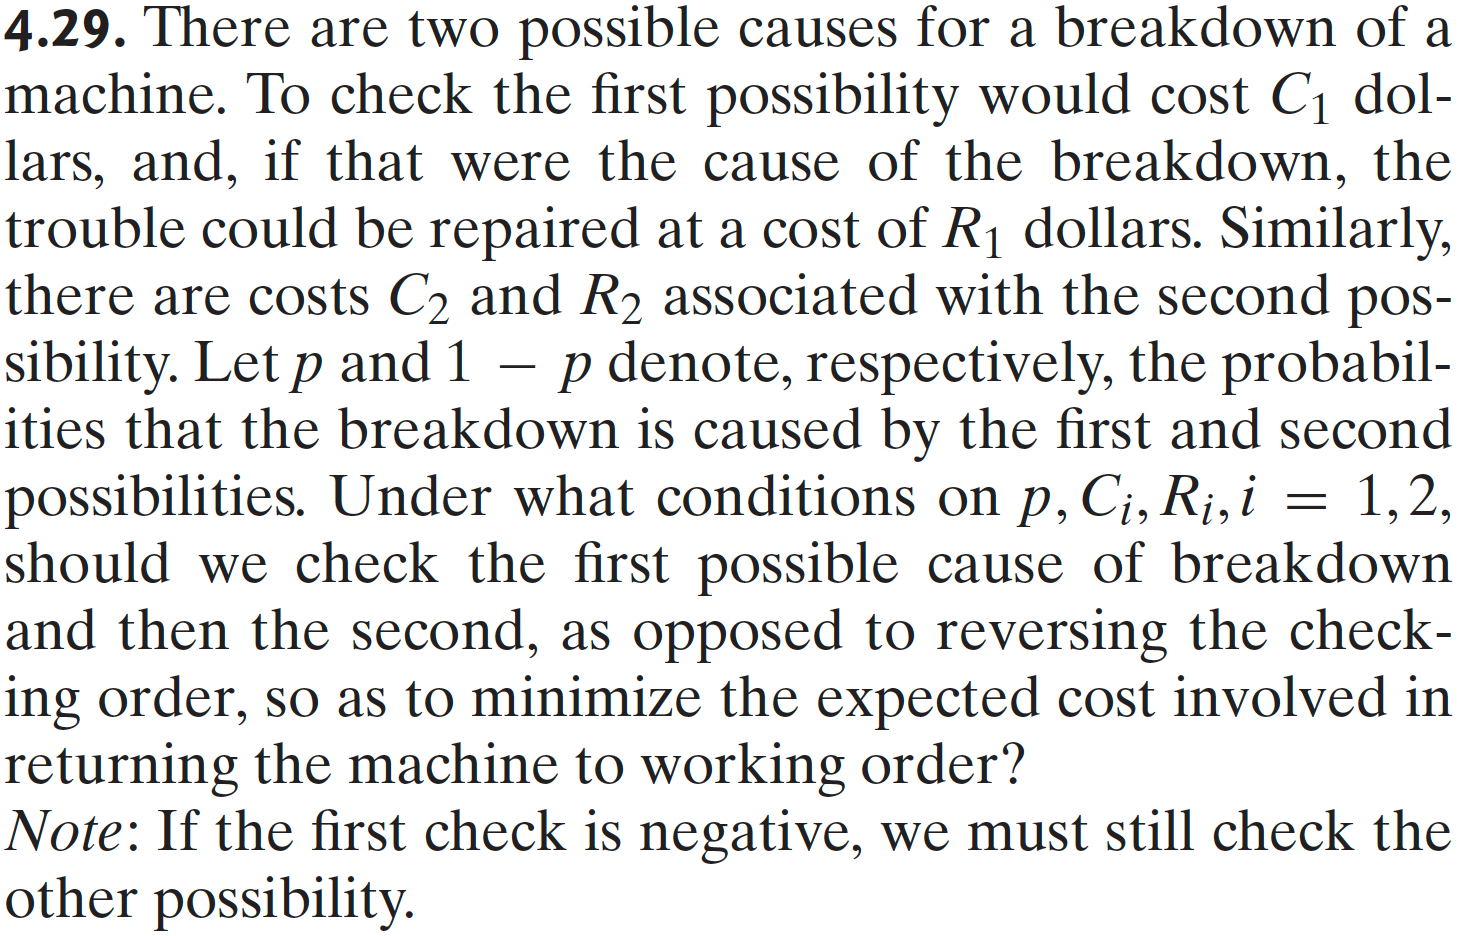
\includegraphics[width=.7\linewidth]{p4_29_p212}
	\newpage
	
	\subsection{Davignon exercice 4.8 p. 91}
	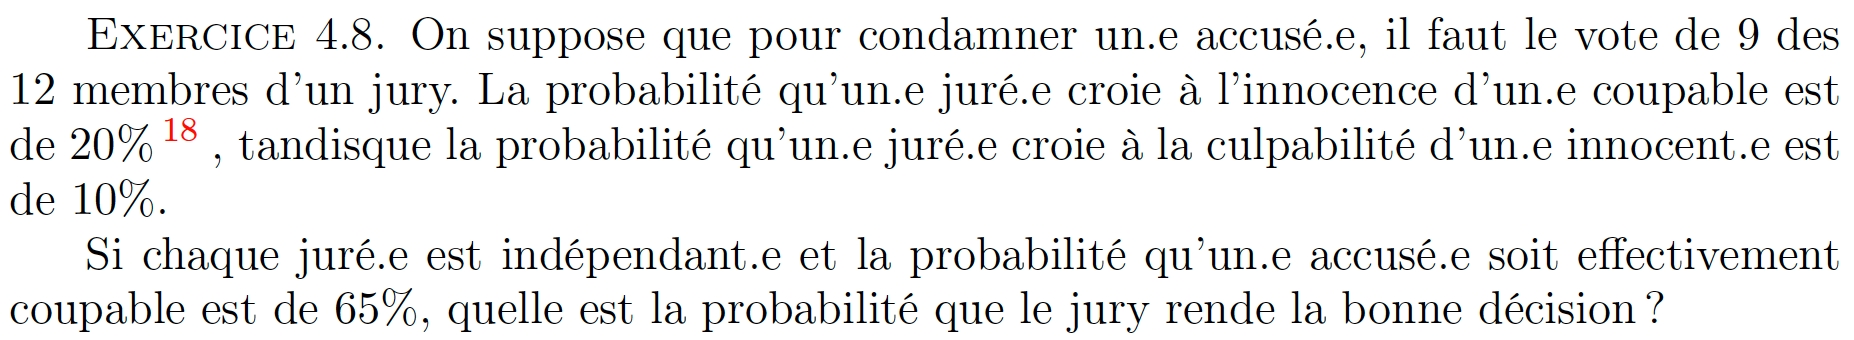
\includegraphics[width=\linewidth]{dvg_4_8_p91}
	\newpage
	
	\section{Chapitre 3 : Probabilité conditionnelle et indépendance}
	\subsection{Ross auto-évaluation 3.13 p. 144}
	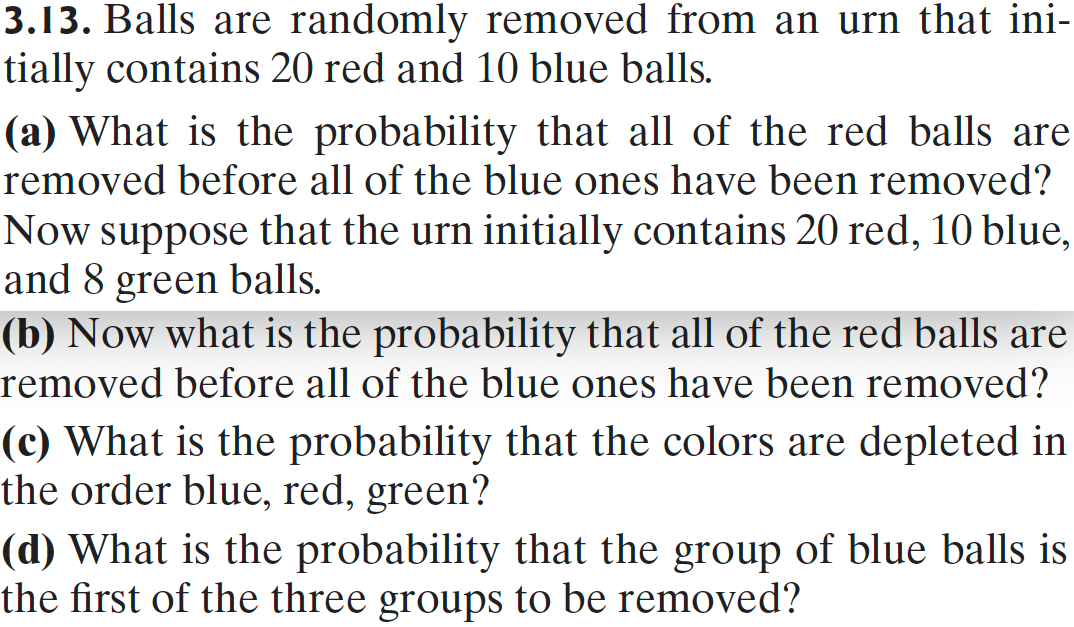
\includegraphics[width=.7\linewidth]{a3_13_p144}
	
\end{document}
